\documentclass{beamer}

\usetheme{Antibes}
\usepackage{pgfplots}
\title[GATE\_PROBLEM]{CONTROL SYSTEMS}
\subtitle{PRESENTATION}
\author{Varun-EE18BTECH11030}
\usepackage{graphicx}
\usepackage{mathpazo}
\usepackage{tikz}
\usetikzlibrary{shapes,arrows}
\usepackage{verbatim}
\usepackage{amsmath}



\begin{document}

\begin{frame}
\titlepage    
\end{frame}

\section{Question}
\begin{frame}{Question 46 EC 2017}
A unity feedback control system is characterised by the open-loop transfer function\\
\begin{centre}
$$
 G(S) = \frac{2(s+1)}{s^3 + ks^2 + 2s +1}
$$
\end{centre}

the value of the k for which the system oscillates at 2 rad/s \\

\end{frame}
\begin{frame}{Unity Feedback Control System Block Diagram}
\begin{centre}


\tikzstyle{block} = [draw, fill=blue!20, rectangle, 
    minimum height=4em, minimum width=8em]
\tikzstyle{sum} = [draw, fill=blue!20, circle, node distance=1.5cm]
\tikzstyle{input} = [coordinate]
\tikzstyle{output} = [coordinate]
\tikzstyle{pinstyle} = [pin edge={to-,thin,black}]

% The block diagram code is probably more verbose than necessary
\begin{tikzpicture}[auto, node distance=3.5cm,>=latex']
    % We start by placing the blocks
    \node [input, name=input] {};
    \node [sum, right of=input] (sum) {};
    \node [block, right of=sum] (controller) {G(s)};
    \node [output, right of=controller] (output) {};
    \node [block, below of=controller] (measurements) {H(s) = 1};

    % Once the nodes are placed, connecting them is easy. 
    \draw [draw,->] (input) -- node {$R(s)\  +$} (sum);
    \draw [->] (sum) -- node {$E(s)$} (controller);
    \draw [->] (controller) -- node [name=y] {$Y(s)$}(output);
    \draw [->] (y) |- (measurements);
    \draw [->] (measurements) -| node[pos=0.99] {$-$} 
        node [near end] {$Y_m(s)$} (sum);
     
\end{tikzpicture}


\end{centre}

    
\end{frame}
\section{Solution}
\begin{frame}{Modelling Closed loop system into a open loop system}
\begin{centre}
$$
E(s) = R(S) - Y_m(s)
$$
$$Y_m(s) = H(s)Y(s)$$
$$
 G(S) = \frac{Y(s)}{E(s)}
$$
$$
 G(S) = \frac{Y(s)}{R(s) - H(s)Y(s)}
$$
$$
 Gm(S) = \frac{Y(S)}{R(s)} = \frac{G(s)}{1 + H(s)G(s)}
$$


\end{centre}
\tikzstyle{block} = [draw, fill=blue!20, rectangle, 
    minimum height=3em, minimum width=6em]
%\tikzstyle{sum} = [draw, fill=blue!20, circle, node distance=1.5cm]
%\tikzstyle{input} = [coordinate]
%\tikzstyle{output} = [coordinate]
%\tikzstyle{pinstyle} = [pin edge={to-,thin,black}]

% The block diagram code is probably more verbose than necessary
\begin{tikzpicture}[auto, node distance=2.5cm,>=latex']
 
    \node [block, right of=sum] (controller) {Gm(s)};
    \node [output, right of=controller] (output) {};
 
    \draw [->] (sum) -- node {$R(s)$} (controller);
    \draw [->] (controller) -- node [name=y] {$Y(s)$}(output);

     
\end{tikzpicture}

\end{frame}
\begin{frame}{Routh's Stability Condition}
\begin{itemize}
   \item If the closed-loop transfer function has all poles in the left half of the s-plane,the system is stable.Thus,a system is stable if there are no sign changes in the first column of the Routh table.
   \item The Routh - Hurwitz criterion declares that the number of roots of the polynomial that are lies in the right half-plane is equal to the number of sign changes in the first column of Routh's array .Hence the system is unstable if the poles lies on the right hand side of the s-plane.
   
\end{itemize}

\end{frame}

\begin{frame}
Characteristic equation : $$1 + G(s)H(s) = 0$$
$$H(s) = 1 $$
$$ 1 + G(s) = 0$$
$$ 1 + \frac{2(s+1)}{s^3 + ks^2 + 2s +1} = 0$$
$$ \frac{s^3+ks^2+4s+3}{s^3 + ks^2 + 2s +1} = 0 $$
$$ s^3+ks^2+4s+3 = 0$$
\end{frame}

\begin{frame}
Characteristic Equation :\\
$$s^3+ks^2+4s+3 = 0$$
Develop Routh's Array :\\
\begin{centre}
\[ \begin{array}{l|c  r}

\mbox S^3 & 1 & 4 \\~\\~\\
\mbox S^2 & k & 3 \\~\\
\mbox S & \frac{\begin{vmatrix}
1 & 4 \\ 
k & 3 \\  
\end{vmatrix}}{k} = \frac{3 - 4k}{k} & 0 \end{array}\] 
\\
\end{centre}
\end{frame}
\begin{frame}
 Given that ,System oscillates at a frequency 2 rad/s \\
\begin{itemize}

   \item If all the coefficients in a row are zero, then auxiliary polynomial has pair of roots of equal magnitude and opposite sign is indicated. These could be two real roots with equal magnitudes and opposite signs or two conjugate imaginary roots.
   \item The auxiliary polynomial, is obtained from the values in the row above the zero row.
   \item Auxiliary polynomial is always even degree.
\end{itemize}

\end{frame}
\begin{frame}
\begin{centre}

$$
\frac{3 - 4k}{k} = 0
$$
$$ k = \frac{3}{4}$$
Auxilary polynomial\\
$$
 ks^2 +3 = 0
$$
$$
 \frac{3}{4}s^2 +3 = 0
$$
$$
 s^2 + 4 =0 
$$
$$  s = \pm 2j$$
Magnitude is 2 rad/sec 


\end{centre}
    
\end{frame}
\begin{frame}
\begin{centre}


Given oscillating frequency $$\omega = 2 rad/s$$ 

$$ T = \frac{2\pi}{\omega}$$
$$T = \frac{2\pi}{2}$$
$$
 T = \pi = 3.14 
$$




\end{centre}
    
\end{frame}
\begin{frame}{Plot}
\begin{figure}
    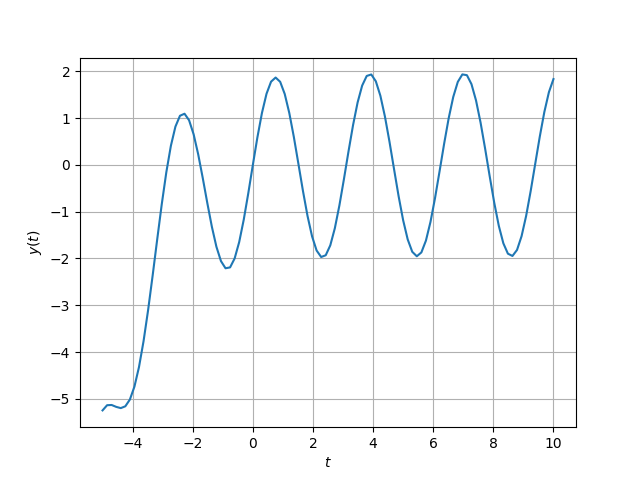
\includegraphics[scale=0.60]{figures/presentation.png}
    
\end{figure}
    
\end{frame}

\end{document}

